\subsection{Background: from GAN to conditional WGAN}

Generative Adversarial Networks (GANs) were originally presented by I.~Goodfellow~\etal in 2014 \cite{goodfellow2014generative} and quickly became a state-of-the-art technique in areas such as image generation \cite{radford2015unsupervised}, with a huge number of extensions \cite{IsolaZZE16,CycleGAN2017,wang2018video}.

In the GAN framework, the aim is to learn a mapping $G$, usually called \textit{generator}, to warp an easy-to-draw distribution $p(\vz)$ (e.g. $p(\vz) = \mathcal{N}(0, I)$) into a target distribution $\pdata(\vx)$ to facilitate sampling from $\pdata(\vx)$. When $G$ is learned, $G \equiv G^*$, sampling from the target distribution $\pdata(\vx)$ is done by first drawing a sample from the distribution $p(\vz)$ and then feeding the sample into the generator: $G^*(\vz) \sim \pdata$, where $\vz \sim p(\vz)$. For such sampling procedure, the time needed to draw a sample from $\pdata(\vx)$ is approximately equal to the time needed to evaluate the function $G$ in a point.  

The generator is learned by using a feedback from an external classifier (usually called \textit{discriminator}), which tries to find discrepancy between the target distribution $\pdata(\vx)$ and fake distribution $\pfake(\vx)$ defined by samples from the generator $G(\vz) \sim \pfake(\vx),\, \vz \sim p(\vz)$. %The process in summarised in~\cref{fig:GANs}.

% \begin{figure}
% \centering
% 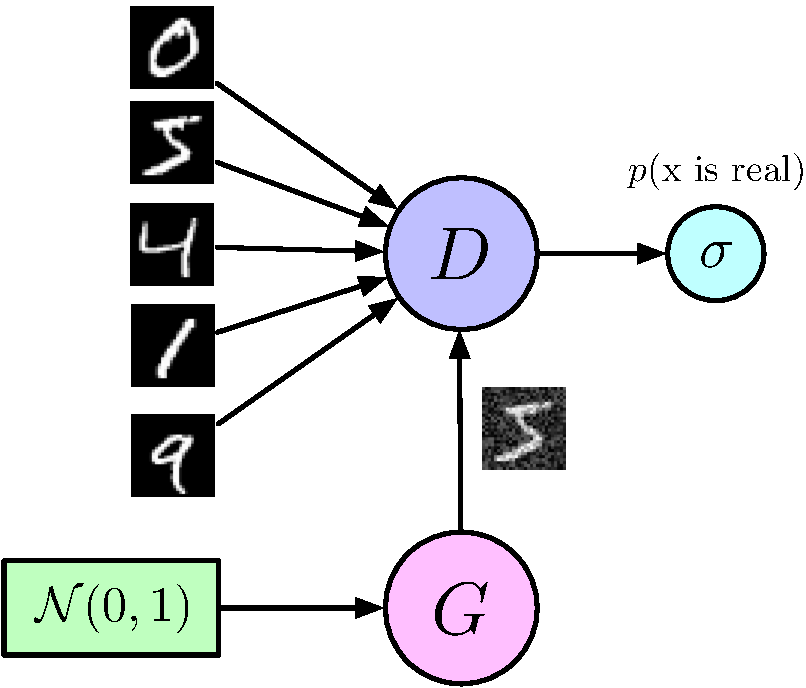
\includegraphics[width=0.3\linewidth]{figures/gan_pic.pdf}
% \caption{Generative Adversarial Networks for digit generation. The generator $G$ transforms the noise vector $\vz \sim p(z)$ to an image of a digit and the discriminator $D$ classifies inputs as real digits or fake digits from generator. Generator and discriminator are trained in an adversarial manner: the task of $G$ is to make it impossible for $D$ to distinguish between the real and fake digits as in this case $G$ reproduces the data distribution $\pdata$.}\label{fig:GANs}
% \end{figure}


More formally, generator $G$ and discriminator $D$ play the following zero sum game: 
\begin{equation}\label{eq:gan}
\min_G \max_D \E_{\vx \sim \pdata(\vx)} [\log D(\vx)] + \E_{\vx \sim \pfake(\vx)} [\log(1 - D(\vx))]\, ,
\end{equation} 
where $D(G(\vz))$ is the output of the discriminator specifying the probability of its input to come from the target distribution $\pdata$.

In practice, the mappings $G$ and $D$ are parametrized by deep neural networks and the objective~\cref{eq:gan} is optimized using alternating gradient descent. For a fixed generator, the discriminator minimizes binary cross-entropy in a binary classification problem (samples from $\pdata$ versus samples from $\pfake$). For the fixed discriminator, the generator is updated to make its samples to be misclassified by the discriminator, thus moving the  fake distribution closer to the target distribution.   

For a fixed generator, it is possible to show that  the optimal value for the inner optimization can be written analytically: 
\begin{equation}\label{eq:js}
\max_D \E_{\vx \sim \pdata(\vx)} [\log D(\vx)] + \E_{\vx \sim \pfake(\vx)} [\log(1 - D(\vx))] = \text{JS}( \pdata \dsep \pfake)\, , 
\end{equation} 
where $\text{JS}$ is the Jensen-Shannon divergence. In fact, for the fixed generator (hence fixed fake distribution), the discriminator computes the divergence between the target distribution $\pdata$ and the fake distribution $\pfake$. When the divergence is computed, the generator aims to update the fake distribution to make this divergence lower: $\min_G \text{JS}( \pdata \dsep \pfake )$. While the Jensen-Shannon divergence naturally arises from the original game~\cref{eq:gan}, any divergence or distance $\mathcal{D}$ can be used instead: $\min_G \mathcal{D}( \pdata \dsep \pfake )$.
A recent work~\cite{arjovsky2017wasserstein} proposed to use the \textit{Wasserstein distance} instead of the Jensen-Shannon divergence proving its better behavior:
\begin{equation}\label{eq:wasserstein_metric}
W(\pdata \dsep \pfake ) = \max_{\f \in \mathcal{F}} \E_{\vx \sim \pdata(\vx)}[\f(\vx)] - \E_{\vx \sim \pfake} [\f(\vx)]
\end{equation}
where $\mathcal{F}$ is a set of 1-Lipshitz functions. Using the Wasserstein distance instead of the Jensen-Shannon divergence in the GAN objective leads to the Wasserstein GAN (WGAN) objective: 
\begin{equation}\label{eq:wgan}
\min_G \max_{\f \in \mathcal{F}} \E_{\vx \sim \pdata(\vx)}[\f(\vx)] - \E_{\vx \sim \pfake(\vx)} [\f(\vx)]\, .
\end{equation}

It is highly non-trivial to search over the set of 1-Lipshitz functions and several ways have been proposed in order to force this constraint \cite{arjovsky2017wasserstein,gulrajani2017improved}. In Ref. \cite{gulrajani2017improved}, it is proved that the set of optimal functions for~\cref{eq:wgan} contains such function, that the norm of it's gradient in any point equals one. In practice, this result motivates an additional loss added to the objective~\cref{eq:wgan} with a weight $\lambda$, while the hard constraint on the function $\f$ to belong to the set $\mathcal{F}$ is removed and $\f$ is searched over all possible functions:    
\begin{equation}\label{gpwgan-loss}
% \begin{gathered}
\min_G \max_\f \E_{\vx \sim \pdata(\vx)}  \f(\vx) - \E_{\vx \sim \pfake(\vx)} \f(\vx) + 
\lambda \E_{\vx \sim \pfake} \big(\|\nabla_{\tilde{\vx}} D(\tilde{\vx})\|_2 - 1\big)^2 .
% \end{gathered}
\end{equation}

WGAN can be easily adapted to model a conditional distribution $\pdata(\vx | \vy)$. The generator is modified to take the condition along with the sample $\vz$ so the fake distribution is now defined as $G(\vz, \vy) \sim \pfake(\vx | \vy),\, \vz \sim p(\vz)$ and the game is 
\begin{equation}\label{CWGAN}
% \begin{gathered}
\min_G \max_\f \E_{\vy \sim p(\vy)} \Big[ \E_{\vx \sim \pdata(\vx | \vy)}  \f(\vx) - \E_{\vx \sim \pfake(\vx | \vy)} \f(\vx) + 
\lambda \E_{\vx \sim \pfake(\vx | \vy)} \big(\|\nabla_{\tilde{\vx}} D(\tilde{\vx})\|_2 - 1\big)^2 \Big]\,.
% \end{gathered}
\end{equation}


% \subsubsection{Wasserstein GAN}
% There are various modifications of GANs for struggling with some typical problems and for improving the training procedure. A common GANs issue is so-called mode collapse when $p_\text{model} (\vx)$ fails to capture a multimodal nature of $\pdata(\vx)$ and in extreme cases all the generated samples might be identical, in more involved architectures such as Wasserstein GAN \cite{arjovsky2017wasserstein} the discriminator loss is argued to be consistent with the image quality. The main idea is to apply the Wasserstein-1 distance in order to compare $\pdata$ and $p_{\text{model}}$.

% Let $\mathbb{X}$ be a compact metric set and let $\mathbb{B}$ denote the set of all the Borel subsets of $\mathbb{X}$. Let $Prob(\mathbb{X})$ denote the space of probability measures defined on $\mathbb{X}$. The \emph{Earth-Mover} or \emph{Wasserstein-1} distance between two distributions $\mathbb{P}_r, \mathbb{P}_g \in Prob(\mathbb{X})$ is defined in the following way:

% \begin{equation}\label{wasserstein_metric}
% W(\mathbb{P}_r, \mathbb{P}_g) = \inf_{\gamma \in \Pi(\mathbb{P}_r, \mathbb{P}_g)} \mathbb{E}_{(x, y) \sim \gamma} \big{[}\|\vx-\textbf{y}\|\big{]},
% \end{equation}

% where $\Pi(\mathbb{P}_r, \mathbb{P}_g)$ is the set of all joint distributions $\gamma(x, y)$ whose marginals are respectively $\mathbb{P}_r$ and $\mathbb{P}_g$. $\gamma(x, y)$ denotes how much “mass” must be transported from $x$ to $y$ in order to transform the distributions $\mathbb{P}_r$ into the distribution $\mathbb{P}_g$. Thus, the Wasserstein distance can be defined as the minimum cost of transporting mass in order to transform the distribution $\mathbb{P}_r$ into the distribution $\mathbb{P}_q$. 

% By applying to this distance the \emph{Kullback--Leibler divergence}, the \emph{Jensen-Shannon divergence} and the Kantorovich--Rubinstein duality and also parameterization of a family of functions $\{f_w\}_{w \in \mathcal{W}}$ that are all K-Lipschitz for some K we could consider solving the problem (for more detailed information see the paper \cite{arjovsky2017wasserstein})

% \begin{equation}\label{optim}
% \max_{w \in \mathcal{W}} \mathbb{E}_{x \sim P_r}[f_w(x)] - \mathbb{E}_{z\sim p(z)} [f_w(g_\theta(z))]
% \end{equation}

% and if the supremum in \eqref{optim} is attained for some $w \in \mathcal{W}$, this process would lead to a calculation of $W(\mathbb{P}_r, \mathbb{P}_\theta)$ up to a multiplicative constant.
% So, the WGAN value function is
% \begin{equation}\label{wgan_loss}
% \min_G \max_{D \in \mathcal{D}}  \mathbb{E}_{\vx \sim \mathbb{P}_r}  [D(\vx)] - \mathbb{E}_{\tilde{\vx} \sim \mathbb{P}_g} [D(\tilde{\vx})],
% \end{equation}
% where $\mathcal{D}$ is the set of 1-Lipschitz functions and $\mathbb{P}_g$ is  the model distribution defined by $\tilde{\vx} = G(\vz), ~\vz \sim p(\vz).$

% In general, the training procedure of GANs is known to be difficult and presents such issues as mode collapse, and WGAN often helps to overcome this problem.

% The Wasserstein GAN value function makes the optimization process easier because the discriminator's gradient with respect to its input is better behaved than its GAN counterpart. Also, it was noticed that the WGAN value function tend to correlate with the original data quality which is not always the case for ordinary GANs.


% \subsubsection{Wasserstain GAN with gradient penalty}
% An alternative way to enforce the Lipschitz constraint was introduced in \cite{gulrajani2017improved}. The authors consider directly constraining the gradient norm of the discriminator's output with respect to its input because a differentiable function is 1-Lipschtiz if and only if it has gradients with norm at most 1 everywhere. To come over tractability issues a soft version of the constraint with a penalty on the gradient norm for random samples $\tilde{\vx} \sim \mathbb{P}_{\tilde{\vx}}$ was suggested. Therefore, a new obtained objective is 
% \begin{equation} \label{gpwgan-loss}
% \begin{gathered}
% \mathcal{L}(\bm{\theta}) =
% \underbrace{ \underset{\tilde{\vx} \sim \mathbb{P}_g}{\mathbb{E}}  \Big[D(\tilde{\vx})\Big] - \underset{\vx \sim \mathbb{P}_r}{\mathbb{E}} \Big[D(\vx)\Big]}_{\text{original loss}} + 
% \underbrace{ \lambda \underset{\vx \sim \mathbb{P}_g}{\mathbb{E}} \Big[\big(\|\nabla_{\tilde{\vx}} D(\tilde{\vx})\|_2 - 1\big)^2 \Big]}_{\text{gradient penalty}}.
% \end{gathered}
% \end{equation}

% This approach demonstrates strong modelling performance and stability across a variety of architectures.  Now it is a state-of-the-art technique in GANs. 
% How to calculate this loss in practice is described on~\cref{sec:training_strategy}.

\subsection{GANs in high energy physics}
A  systematic study on the application of deep learning to the simulation of calorimeters for particle physics has been carried out by Paganini et al. in 2017~\cite{paganini2017calogan} and has resulted in the CaloGAN package. The authors aim to speed up particle simulation in a 3-layer heterogeneous calorimeter using GANs framework and achieve $\sim \times 10^5 $ speedup. They used an existing state-of-the-art but slow simulation engine \geant to create a training dataset. They simulated positrons, photons and charged pions with various energies sampled from a flat distribution between 1 GeV and 100 GeV. All incident particles in this study have an initial momentum perpendicular to the face of the calorimeter. The shower in the first layer is represented as a $3 \times 96$ pixel image, the middle layer as a $12 \times 12$ pixel image, and the last layer as a $12 \times 6$ pixel image. 

Their design of the generator network is based on a DCGAN structure \cite{radford2015unsupervised} with some convolutional layers replaced by locally-connected layers \cite{taigman2014deepface}. The idea of locally connected layers is based on the fact that every pixel position gets its own filter while an ordinary convolutional layer is applied over the whole image, independently of location. An extension of this method to particle physics simulation has been described in the previous work of the authors, where the resulting type of neural network was called LAGAN \cite{de2017learning}. A special section in the paper is devoted to the evaluation of the quality of the CaloGAN produced images, where the sparsity level,  energy per layer or total energy, are used as measures of the performance of the model. 

The obtained results demonstrate a prospect of application of GANs for the particle showers generation and its replacement of the Monte Carlo methods with the proposed approach. The CaloGAN approach yields sizeable simulation-time speedups compared to \geant. 

%In fact, the CaloGan model is based on DCGAN with the described tricks. However, GANs tend to suffer from mode collapse. Therefore, the CaloGan architecture cannot be applied for all datasets, because %here is a high probability of mode collapse appearance and it is a limitation of this work.
